\chapter{Introduction}
\paragraph{}As previously mentioned, deep learning combines feature extraction through convolution and pooling with traditional neural networks, eliminating the need for humans to manually extract features from datasets. Convolution, in essence, is a filtering process where trained filter(s) slides over the input data to extract features and other useful information. Pooling is the subsequent process of taking local samples and selecting either the minimum, maximum, or average of those samples. This step helps identify feature locations and condenses the information produced by the convolution layer.

\paragraph{}A typical deep learning pipeline consists of several convolution and pooling layers, followed by a few fully connected layers. In this work, we aim to demonstrate that using a deep learning network configuration can reduce the size of the feed-forward section without compromising program classification performance, thereby highlighting the effectiveness of deep learning.

\paragraph{}The MNIST database is a standard benchmark for image-processing neural networks. For our comparison, we will use a modified version of the DLIB deep learning example. This approach allows us to showcase the differences between standard feed-forward neural networks and deep learning networks without requiring expensive GPUs or AI accelerators. While the MNIST dataset is solvable using only feed-forward neural networks, we intend to demonstrate that feature extraction with deep learning can achieve better prediction accuracy, even with smaller classification networks.

\chapter{Experimental Setup}
\paragraph{}
The MNIST database comprises grayscale images of size 28x28 pixels, with 60,000 training images and 10,000 test images. For each experiment, we present graphs comparing the average error per epoch for both configurations, alongside a table summarizing the test results of the final network after training. Due to resource constraints, training is limited to a maximum of 100 epochs, and the experiments are averaged over ten runs. Notably, the deep learning configuration requires approximately six hours to complete on a 32-thread workstation.

\paragraph{}
Our experiments are divided into two phases, each testing a deep learning network alongside its corresponding feed-forward network. To ensure a fair comparison, the feed-forward test focuses exclusively on the feed-forward component of the deep learning network. This approach ensures consistency in variables such as the number of layers or nodes in the feed-forward section, minimizing potential biases and preserving the integrity of the results.

\section{Experiment 1}
\paragraph{}
The first experiment compares the performance of a deep learning configuration to a baseline feed-forward network, using the example provided in the DLIB C++ library. The deep learning configuration consists of two ReLU-activated convolutional layers, each followed by max-pooling and then a fully connected feed-forward network.

\paragraph{}
The first convolutional layer uses six filters, each sized 5x5, with a stride of 1x1. The second convolutional layer applies sixteen filters with the same size and stride configuration. After each convolutional operation, the output is passed through a max-pooling layer with a filter size of 2x2 and a stride of 2x2, which reduces the spatial dimensions.

\paragraph{}
The pooled features are then fed into a three-layer fully connected ReLU-activated feed-forward network. The fully connected layers consist of 120 neurons in the first layer, 84 neurons in the second, and 10 neurons in the final output layer, with each output representing a predicted class for the input image.

\paragraph{}
For comparison, the baseline configuration omits the convolutional and pooling layers and consists solely of the three-layer feed-forward network. This setup isolates the feed-forward network’s performance, enabling a direct comparison with the deep learning configuration.

\begin{figure}[H]
	\centering
	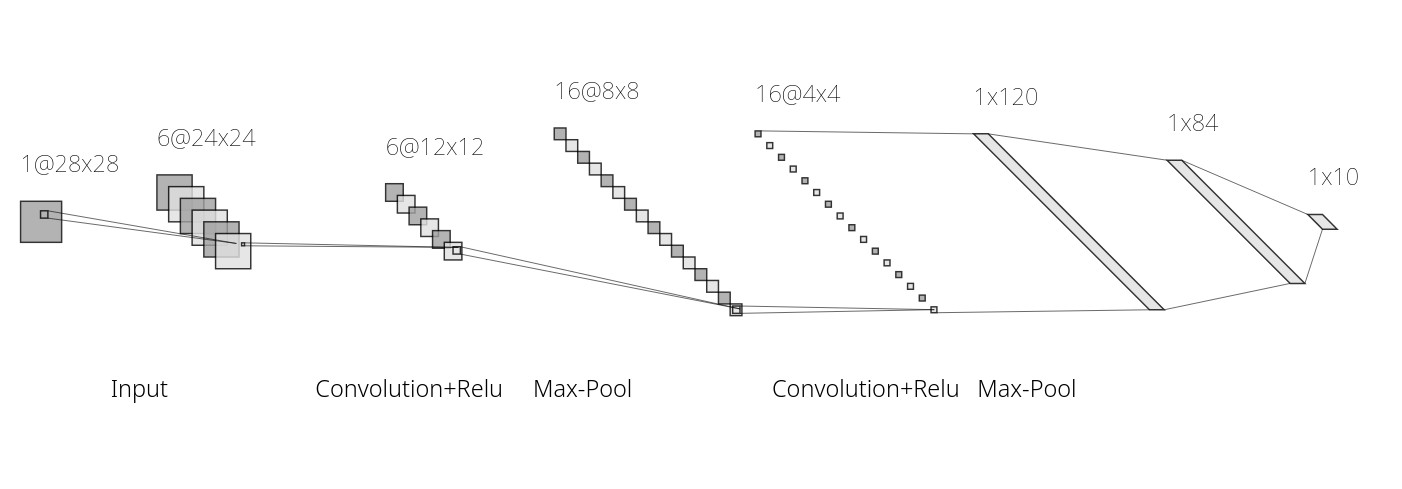
\includegraphics[width=\linewidth]{screenshot003}
	\caption{Experiment 1 network configuration.}
	\label{fig:screenshot003}
\end{figure}


\section{Experiment 2}
\paragraph{}
The second experiment retains the same convolutional and pooling configurations as in Experiment 1 but modifies the number of neurons in the feed-forward section of the network. This adjustment reduces the number of parameters available for object detection and classification, allowing for an evaluation of how deep learning's hierarchical feature extraction compensates for reduced network capacity.

\paragraph{}
By demonstrating the impact of parameter constraints, this experiment highlights the advantage of feature extraction in the deep learning configuration, particularly when resources in the feed-forward section are limited. This serves to underscore the practical utility of convolutional layers in achieving robust classification performance with smaller, more efficient networks.

\begin{figure}[H]
	\centering
	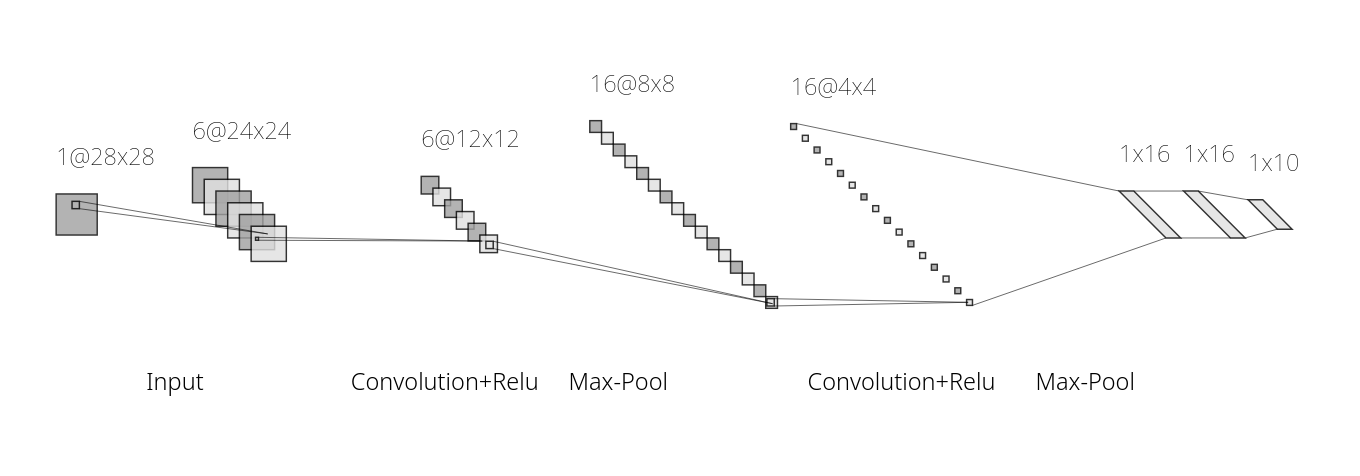
\includegraphics[width=\linewidth]{screenshot004}
	\caption{Experiment 2 network configuration.}
	\label{fig:screenshot004}
\end{figure}
